\documentclass[a4paper,12pt]{report}
\setcounter{secnumdepth}{5}
\setcounter{tocdepth}{3}
\input{/usr/share/LaTeX-ToolKit/template.tex}
\begin{document}
\title{Hyperbolic Functions}
\author{沈威宇}
\date{\temtoday}
\titletocdoc
\renewcommand{\arraystretch}{1.5}
\sct{Hyperbolic Functions (雙曲函數)}
\ssc{Hyperbolic Functions}
\sssc{Definition}
\begin{longtable}[c]{|p{0.16\textwidth}|p{0.16\textwidth}|p{0.16\textwidth}|p{0.16\textwidth}|p{0.16\textwidth}|}
\hline
Function & Symbols & Definition & Domain & Range \\
\hline\endhead
    Hyperbolic sine (雙曲正弦) & $\sinh x$ & $\frac{e^{x}-e^{-x}}{2}$ & $\bbR$ & $\bbR$ \\\hline
    Hyperbolic cosine (雙曲餘弦) & $\cosh x$ & $\frac{e^{x}+e^{-x}}{2}$ & $\bbR$ & $(1,\infty)$ \\\hline
    Hyperbolic tangent (雙曲正切) & $\tanh x$ & $\frac{\sinh(x)}{\cosh(x)}$ & $\bbR$ & $(-1,1)$ \\\hline
    Hyperbolic cotangent (雙曲餘切) & $\coth x$ & $\frac{\cosh(x)}{\sinh(x)}$ & $\bbR\setminus\{0\}$ & $(-\infty,-1)\cup(1,\infty)$ \\\hline
    Hyperbolic secant (雙曲正割) & $\sech x$ & $\frac{1}{\cosh(x)}$ & $\bbR$ & $(0,1]$ \\\hline
    Hyperbolic cosine (雙曲餘弦) & $\cosh x$ & $\frac{1}{\sinh(x)}$ & $\bbR\setminus\{0\}$ & $\bbR\setminus\{0\}$ \\\hline
\end{longtable}
\FB
\sssc{Power notation}
\[\ba
&\sinh^n x\coloneq\begin{cases}\qty(\sinh x)^n,\quad n\geq 0\\\arcsinh x,\quad n=-1\end{cases}\\
&\cosh^n x\coloneq\begin{cases}\qty(\cosh x)^n,\quad n\geq 0\\\arccosh x,\quad n=-1\end{cases}\\
&\tanh^n x\coloneq\begin{cases}\qty(\tanh x)^n,\quad n\geq 0\\\arctanh x,\quad n=-1\end{cases}\\
&\coth^n x\coloneq\begin{cases}\qty(\coth x)^n,\quad n\geq 0\\\arccoth x,\quad n=-1\end{cases}\\
&\sech^n x\coloneq\begin{cases}\qty(\sech x)^n,\quad n\geq 0\\\arcsech x,\quad n=-1\end{cases}\\
&\csch^n x\coloneq\begin{cases}\qty(\csch x)^n,\quad n\geq 0\\\arccsch x,\quad n=-1\end{cases}
\ea\]
\ssc{Inverse hyperbolic function (反雙曲函數)}
\sssc{Definition}
\begin{longtable}[c]{|p{0.16\textwidth}|p{0.16\textwidth}|p{0.16\textwidth}|p{0.16\textwidth}|p{0.16\textwidth}|}
\hline
Function & Symbols & Definition & Domain & Range \\
\hline\endhead
    Inverse hyperbolic sine (反雙曲正弦) & \(y=\arcsinh x=\sinh^{-1}(x)=\asinh(x)\) & \(x=\sinh y\) & \(\bbR\) & \(\bbR\) \\ \hline
    Inverse hyperbolic cosine (反雙曲餘弦) & \(y=\arccosh x=\cosh^{-1}(x)=\acosh(x)\) & \(x=\cosh y\) & \([1,\infty)\) & \([0,\infty)\) \\ \hline
    Inverse hyperbolic tangent (反雙曲正切) & \(y=\arctanh x=\tanh^{-1}(x)=\atanh(x)\) & \(x=\tanh y\) & \((-1,1)\) & $\bbR$ \\ \hline
    Inverse hyperbolic cotagent (反雙曲餘切) & \(y=\arccoth x=\coth^{-1}(x)=\acoth(x)\) & \(x=\coth y\) & \((-\infty,-1)\cup(1,\infty)\) & \(\bbR\setminus\{0\}\) \\ \hline
    Inverse hyperbolic secant (反雙曲正割) & \(y=\arcsech x=\sech^{-1}(x)=\asech(x)\) & \(x=\sech y\) & \((0,1]\) & $[0,\infty)$ \\ \hline
    Inverse hyperbolic cosecant (反雙曲餘割) & \(y=\arccsch x=\csch^{-1}(x)=\acsch(x)\) & \(x=\csch y\) & \(\bbR\setminus\{0\}\) & \(\bbR\setminus\{0\}\) \\ \hline
\end{longtable}
\FB
\sssc{Logarithmatic forms}
\bma
\operatorname{arcsinh} &= \ln\left(x+\sqrt{x^2+1}\right)\\
\operatorname{arccosh} &= \ln\left(x+\sqrt{x^{2}-1}\right),\quad x\geq 1\\
\operatorname{arctanh} &= \frac{1}{2}\ln\left(\frac{1+x}{1-x}\right),\quad\abs{x}<1\\
\operatorname{arccoth} &= \frac{1}{2}\ln\left(\frac{x+1}{x-1}\right),\quad\abs{x}>1\\
\operatorname{arcsech} &= \ln\left(\frac{1}{x}+\frac{\sqrt{1-x^2}}{x}\right),\quad 0<x\leq 1\\
\operatorname{arccsch} &= \ln\left(\frac{1}{x}+\frac{\sqrt{1+x^2}}{\abs{x}}\right),\quad x\neq 0
\eam
\sssc{Hyperbolic functions of inverse hyperbolic functions}
\begin{longtable}[c]{|m{0.1\textwidth}|m{0.12\textwidth}|m{0.12\textwidth}|m{0.12\textwidth}|m{0.12\textwidth}|m{0.12\textwidth}|m{0.12\textwidth}|}
\hline
    \theta & \sinh\theta & \cosh\theta & \tanh\theta & \coth\theta & \sech\theta & \csch\theta \\\hline\endhead
    \arcsinh(x) & x & \sqrt{1+x^2} & \frac{x}{\sqrt{1+x^2}} & \frac{\sqrt{1+x^2}}{x},\quad x\neq 0 & \frac{1}{\sqrt{1+x^2}} & \frac{1}{x},\quad x\neq 0 \\\hline
    \arccosh(x) & \sqrt{x^2-1} & x & \frac{\sqrt{x^2-1}}{x} & \frac{x}{\sqrt{x^2-1}} & \frac{1}{x} & \frac{1}{\sqrt{x^2-1}} \\\hline
    \arctanh(x) & \frac{x}{\sqrt{1-x^2}} & \frac{1}{\sqrt{1-x^2}} & x & \frac{1}{x},\quad x\neq 0 & \sqrt{1-x^2} & \frac{\sqrt{1-x^2}}{x},\quad x\neq 0 \\\hline
    \arccoth(x) & \frac{1}{\sqrt{x^2-1}} & \frac{|x|}{\sqrt{x^2-1}} & \frac{1}{x} & x & \frac{\sqrt{x^2-1}}{|x|} & \sqrt{x^2-1} \\\hline
    \arcsech(x) & \frac{\sqrt{1-x^2}}{x} &{{{ \frac{1}{x} & \sqrt{x^2-1}\operatorname{sgn}\qty(x) & \frac{\operatorname{sgn}\qty(x)}{\sqrt{x^2-1}},\quad|x|>1 & x & \frac{|x|}{\sqrt{x^2-1}} \\\hline
    \arccsc(x) & \frac{1}{x} & \frac{\sqrt{x^2-1}}{|x|} & \frac{\operatorname{sgn}\qty(x)}{\sqrt{x^2-1}},\quad|x|>1 & \sqrt{x^2-1}\operatorname{sgn}\qty(x) & \frac{|x|}{\sqrt{x^2-1}} & x \\\hline
\end{longtable}\FB
\ssc{Identities}
\sssc{雙曲函數基本關係}
\begin{center}
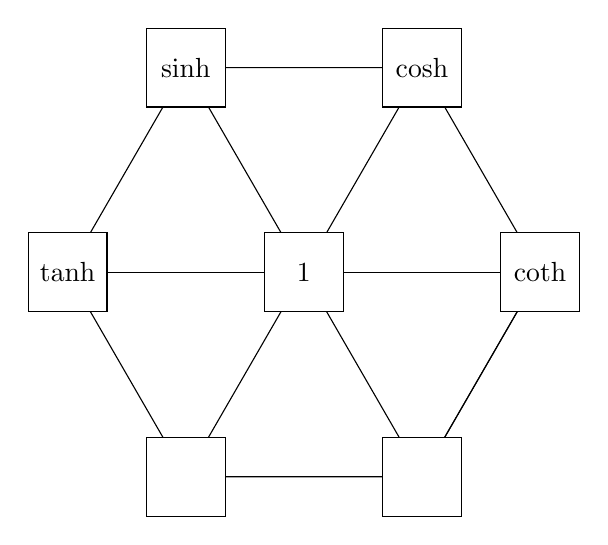
\begin{tikzpicture}
  \foreach \a in {0,60,...,300}
    \node (P\a) at (\a:3) {};
  \draw (P0) -- (P60) -- (P120) -- (P180) -- (P240) -- (P300) -- (P0) -- cycle;
  \draw (P0) -- (P180);
  \draw (P60) -- (P240);
  \draw (P120) -- (P300);
  \draw (P0) -- (P300);
  \node[draw, fill=white, minimum size=1cm, anchor=center] at (P0) {$\coth$};
  \node[draw, fill=white, minimum size=1cm, anchor=center] at (P60) {$\cosh$};
  \node[draw, fill=white, minimum size=1cm, anchor=center] at (P120) {$\sinh$};
  \node[draw, fill=white, minimum size=1cm, anchor=center] at (P180) {$\tanh$};
  \node[draw, fill=white, minimum size=1cm, anchor=center] at (P240) {$\sech$};
  \node[draw, fill=white, minimum size=1cm, anchor=center] at (P300) {$\csch$};
  \node[draw, fill=white, minimum size=1cm, anchor=center] at (0,0) {$1$};
\end{tikzpicture}
\end{center}
\bit
\item 名稱:左側三者為正;右側三者為餘;上面二者為弦;中間二者為切;下面二者為割。
\item 倒數關係:三條通過中心點的線,其兩端者互為倒數,相乘為1。
\item 商數關係:六邊形周上,連續三個頂點形成的連線,其兩端者相乘等於中間者。
\item 平方關係:圖中有三個倒正三角形,其在右上頂點者之平方減去在左上頂點者之平方等於在下方頂點者之平方。
\eit
\sssc{正切萬能公式}
\[\sinh\theta=\frac{2\tanh\frac{\theta}{2}}{1-\tanh^2\frac{\theta}{2}}\]
\[\cosh\theta=\frac{1+\tanh^2\frac{\theta}{2}}{1-\tanh^2\frac{\theta}{2}}\]
\[\tanh\theta=\frac{2\tanh\frac{\theta}{2}}{1+\tanh^2\frac{\theta}{2}}\]



















\end{document}

